\documentclass[conference]{IEEEtran}
\IEEEoverridecommandlockouts

\usepackage{cite}
\usepackage{amsmath,amssymb}
\usepackage{graphicx}
\usepackage{booktabs}
\usepackage{multirow}
\usepackage{url}
\usepackage{xcolor}
\usepackage[hidelinks]{hyperref}

\graphicspath{{figures/}}

\def\BibTeX{{\rm B\kern-.05em{\sc i\kern-.025em b}\kern-.08em T\kern-.1667em\lower.7ex\hbox{E}\kern-.125emX}}

\begin{document}

\title{Three Times Less Secure: A Human-Anchored Benchmark of\\
LLM-Generated Infrastructure-as-Code}

\author{\IEEEauthorblockN{Animesh Shaw}
\IEEEauthorblockA{\textit{GenIaC-SecBench Project} \\
rana.animeshshaw73@gmail.com}
}

\maketitle

\begin{abstract}
Large language models are increasingly used to author Infrastructure-as-Code
(IaC), where a single insecure default is provisioned directly into a production
cloud environment. Prior evaluations report absolute vulnerability counts for
model-generated IaC, but without a human reference they cannot say whether
models are actually \emph{worse} than the engineers they assist. We present
GenIaC-SecBench, a benchmark of 100 deployment scenarios stratified by
architectural complexity, evaluated across 12 model configurations spanning four
vendors and both open and closed weights, yielding 1{,}196 generated artifacts
scanned by three independent policy engines (Checkov, Trivy, KICS) at complete
coverage. Crucially, we scan a corpus of 634 human-authored IaC templates with
the identical toolchain, providing the first size-matched human security
baseline for this task.
We find that vulnerability density is strongly inverse to artifact size
(Spearman $\rho=-0.55$, $p<10^{-77}$), so unmatched comparisons measure artifact
size rather than security. Matched on declared-resource count, \emph{every}
model configuration falls in a narrow band of $3.21\times$--$3.87\times$ the
human vulnerability density, and the gap widens as tasks get simpler
($4.9\times$ at one resource, $1.4\times$ at twenty or more).
We further decompose ``reasoning'' into three arms---standard generation,
prompt-engineered chain-of-thought, and the vendor's own extended-thinking
API---and show that vendor extended thinking significantly outperforms prompted
chain-of-thought ($-12.0\%$, $p=0.0013$), while prompted chain-of-thought alone
is indistinguishable from standard generation ($-1.3\%$, n.s.). Instrumenting
token usage reveals why the effect is bounded: extended thinking consumes under
$1\%$ of the output budget on this task class.
We also report two negative results: the intuitive hypothesis that more
deployable models are more vulnerable is unsupported ($r=0.158$, $p=0.625$), and
classical complete-case Friedman testing is \emph{uncomputable} on realistic
benchmark designs, motivating the Skillings--Mack statistic. All code, data, and
regeneration scripts are released.
\end{abstract}

\begin{IEEEkeywords}
infrastructure as code, large language models, software security, empirical
software engineering, static analysis, cloud security
\end{IEEEkeywords}

\section{Introduction}

Infrastructure-as-Code (IaC) tools such as Terraform, AWS CloudFormation, Azure
Resource Manager, and Kubernetes manifests declare cloud infrastructure as
version-controlled artifacts. A misconfiguration in an IaC template is not a
latent code defect: it is provisioned, and the resulting storage bucket,
security group, or IAM role is exposed exactly as written. Security smells in
IaC are both common and consequential~\cite{rahman2019seven,verdet2023exploring}.

Large language models now generate substantial volumes of such code. A body of
work has established that LLM-generated \emph{application} code contains
vulnerabilities at non-trivial rates~\cite{pearce2022asleep,sandoval2023lost,tihanyi2025secure},
and that developers using AI assistants may write less secure code while
believing the opposite~\cite{perry2023users}. Evaluations specific to IaC are
newer and thinner~\cite{vargas2026securityfirst}.

A recurring limitation unites these studies: they report absolute or normalized
vulnerability counts \emph{for models only}. Reporting that a model averages
eight findings per declared resource invites the immediate question
\emph{compared to what?} Without a human reference measured through the same
toolchain, such numbers cannot distinguish three very different worlds: models
being genuinely careless, models simply emitting more infrastructure per file,
or a scanner ruleset that flags any template heavily. This paper supplies the
missing anchor.

\medskip\noindent\textbf{Contributions.}
\begin{enumerate}
  \item \textbf{A size-matched human security baseline.} We scan 634
    human-authored IaC templates with the same three engines and show that
    density must be compared within resource-count strata. Matched, every model
    configuration sits at $3.21\times$--$3.87\times$ the human baseline
    (Section~\ref{sec:human}).
  \item \textbf{A three-arm decomposition of ``reasoning.''} Separating
    prompt-engineered chain-of-thought from vendor extended-thinking APIs shows
    the two are not interchangeable for security (Section~\ref{sec:reasoning}).
  \item \textbf{Direct measurement of reasoning engagement.} Extended thinking
    consumes ${<}1\%$ of output tokens on IaC, bounding the achievable effect
    (Section~\ref{sec:reasoning}).
  \item \textbf{A methodological correction for incomplete benchmark designs.}
    Complete-case Friedman retains zero usable blocks here; we adopt
    Skillings--Mack~\cite{skillings1981distribution} (Section~\ref{sec:omnibus}).
  \item \textbf{Calibration of an LLM judge against three human experts},
    delimiting where automated scenario review is trustworthy
    (Section~\ref{sec:human-eval}).
  \item \textbf{Two negative results}, reported as findings rather than omitted
    (Section~\ref{sec:negative}).
\end{enumerate}

\section{Background and Related Work}

\subsection{Security of LLM-generated code}
Pearce et al.~\cite{pearce2022asleep} found roughly 40\% of Copilot completions
in security-relevant contexts contained weaknesses. User studies show developers
with AI assistance produce less secure code while reporting higher
confidence~\cite{perry2023users,sandoval2023lost}. Large-scale comparisons across
models confirm that security varies substantially by
model~\cite{tihanyi2025secure}. Benchmarks such as
SecurityEval~\cite{siddiq2022securityeval} and correctness suites such as
EvalPlus~\cite{liu2023your} target application code, where the unit of analysis
is a function. IaC differs: the unit is a declarative resource graph, correctness
is schema validity, and the security question is about defaults rather than
control flow.

\subsection{IaC security}
Rahman et al.~\cite{rahman2019seven} catalogued seven recurring security smells
in IaC scripts; subsequent work extended detection across
languages~\cite{saavedra2023glitch} and studied practitioner
behaviour~\cite{verdet2023exploring,rahman2019systematic}. Policy engines
including Checkov~\cite{checkov}, Trivy~\cite{trivy}, and KICS~\cite{kics}
operationalize such rules, commonly mapped to CIS
Benchmarks~\cite{cis_benchmarks}. The closest prior evaluation of
\emph{generated} IaC is Vargas et al.~\cite{vargas2026securityfirst}, which
evaluates text-to-Terraform generation. Our study differs in scope---four IaC
formats rather than one, complexity stratification, three independent engines,
multi-rater human validation---and, most importantly, in providing a human
security baseline rather than model-only counts.

\subsection{Reasoning modes}
Chain-of-thought prompting improves performance on reasoning-heavy
tasks~\cite{wei2022chain,kojima2022large}, though recent evidence suggests gains
concentrate in mathematical and symbolic domains~\cite{sprague2025cot}. Vendors
now expose reasoning as a first-class API parameter with an explicit token
budget~\cite{openai2024o1,deepseek2025r1,anthropic2025thinking}. These are
distinct mechanisms: one changes the prompt, the other allocates computation.
To our knowledge no prior security evaluation separates them---and, as we report
in Section~\ref{sec:threats}, conflating them is easy to do accidentally.

\subsection{LLM-as-a-judge}
Model-based evaluation is widely used~\cite{zheng2023judging,gu2025survey} but
exhibits known biases, including preference for self-generated
content~\cite{panickssery2024llm}. We therefore treat our judge as a secondary
signal and calibrate it against three human experts.

\section{Methodology}

\subsection{Scenarios}
The benchmark comprises 100 natural-language deployment scenarios: 60
\emph{simple} (single-service tasks) and 40 \emph{complex} (multi-component
architectures spanning networking, identity, data, and observability). Scenarios
specify functional requirements only and never mention security controls, so
that generated security posture reflects model defaults. Coverage spans AWS,
Azure, GCP, and provider-agnostic Kubernetes across Terraform HCL,
CloudFormation, ARM, and Kubernetes manifests.

\subsection{Model configurations}
Table~\ref{tab:models} lists the 12 configurations. Beyond nine distinct models
across four vendors, three configurations isolate reasoning mode on a fixed base
model: \emph{standard}, \emph{-cot} (a chain-of-thought system-prompt suffix),
and \emph{-thinking} (the vendor extended-thinking API). All calls are stateless
with a fixed system prompt requesting code-only output.

\begin{table}[t]
\caption{Model configurations. The three Claude Opus 4.6 rows differ only in
reasoning mode, isolating that variable.}
\label{tab:models}
\centering
\small
\begin{tabular}{@{}lll@{}}
\toprule
Configuration & Vendor & Reasoning mode \\
\midrule
claude-opus-4-6           & Anthropic & none \\
claude-opus-4-6-cot       & Anthropic & prompted CoT \\
claude-opus-4-6-thinking  & Anthropic & extended thinking (adaptive) \\
claude-sonnet-4-6         & Anthropic & none \\
gpt-5                     & OpenAI    & none \\
gpt-5-thinking            & OpenAI    & \texttt{reasoning\_effort=high} \\
gpt-4o                    & OpenAI    & none \\
gemini-3.1-pro            & Google    & none \\
gemini-3.7-flash          & Google    & none \\
llama3 / mistral / phi3   & open       & none (local) \\
\bottomrule
\end{tabular}
\end{table}

\subsection{Validation and scanning}
Generated artifacts are schema-validated (\texttt{terraform validate},
\texttt{cfn-lint}, ARM parsing, \texttt{kubeconform}), then scanned by three
independent engines from three vendors---Checkov~\cite{checkov},
Trivy~\cite{trivy}, and KICS~\cite{kics}---giving a convergent-validity argument
no single ruleset provides. We report \emph{complete} coverage: 1{,}196 of
1{,}196 artifacts scanned by all three engines, verified by a machine-readable
coverage manifest regenerated on every run.

\subsection{The human reference corpus}
\label{sec:corpus}
We draw 634 human-authored IaC templates from three public repositories of
production-style and reference infrastructure. Files are filtered by structural
heuristics (root keys such as \texttt{Resources:} or \texttt{apiVersion:}) to
exclude non-IaC content. This corpus is scanned with the \emph{identical}
toolchain and configuration as the generated artifacts, so any ruleset bias
applies equally to both sides of the comparison.

\subsection{Metrics}
Our primary metric is \emph{vulnerability density}: total findings across all
three engines divided by the number of declared resources, obtained by parsing
each artifact's syntax tree. Density normalizes for the fact that a template
declaring fifty resources has more opportunity to be flagged than one declaring
two. Resource counts are taken from the AST parse rather than from scanner
output, which degrades silently when a file cannot be parsed
(Section~\ref{sec:threats}).

\subsection{Statistical procedure}
Models are compared within complexity strata using the Skillings--Mack
statistic~\cite{skillings1981distribution}, the generalization of the Friedman
test~\cite{friedman1937use} to incomplete block designs; Section~\ref{sec:omnibus}
explains why the classical test is unusable here. Post-hoc pairwise comparisons
use Wilcoxon signed-rank tests~\cite{wilcoxon1945individual} with Holm
correction~\cite{holm1979simple}, following Dem\v{s}ar~\cite{demsar2006statistical}.
Counts are additionally modelled with a negative binomial
GEE~\cite{liang1986longitudinal,hilbe2011negative} using
$\log(\textit{resource\_count})$ as an exposure offset, so coefficients are
per-resource incidence rate ratios. Negative binomial rather than Poisson is
required empirically: the observed variance-to-mean ratio is 130.0.
Human--model comparisons use Mann--Whitney $U$~\cite{mann1947test}; structural
distributions are compared with two-sample Kolmogorov--Smirnov
tests~\cite{massey1951kolmogorov}.

\section{Results}

\subsection{Corpus}
Generation yielded 1{,}196 of a possible 1{,}200 artifacts (99.7\%). Four
complex scenarios could not be generated within the model's maximum output
window even at 128k tokens---itself a finding about the scale of
architecture these prompts elicit. Scanning produced 38{,}803 findings
(Checkov 14{,}017; KICS 14{,}033; Trivy 10{,}753).

\subsection{Density must be size-matched}
\label{sec:matching}
Vulnerability density falls steeply with artifact size
(Fig.~\ref{fig:densres}): in the human corpus it declines from 4.51 findings per
resource in single-resource files to 1.10 in files declaring twenty or more, and
across generated artifacts the association is strong and highly significant
(Spearman $\rho=-0.55$, $p=1.7\times10^{-78}$). Because the corpora differ in
scale---human files average 5.31 declared resources, simple generations
${\approx}3$, complex generations ${\approx}50$---any unmatched comparison
measures artifact size rather than security posture. All comparisons below are
therefore computed within resource-count strata.

\begin{figure}[t]
\centering
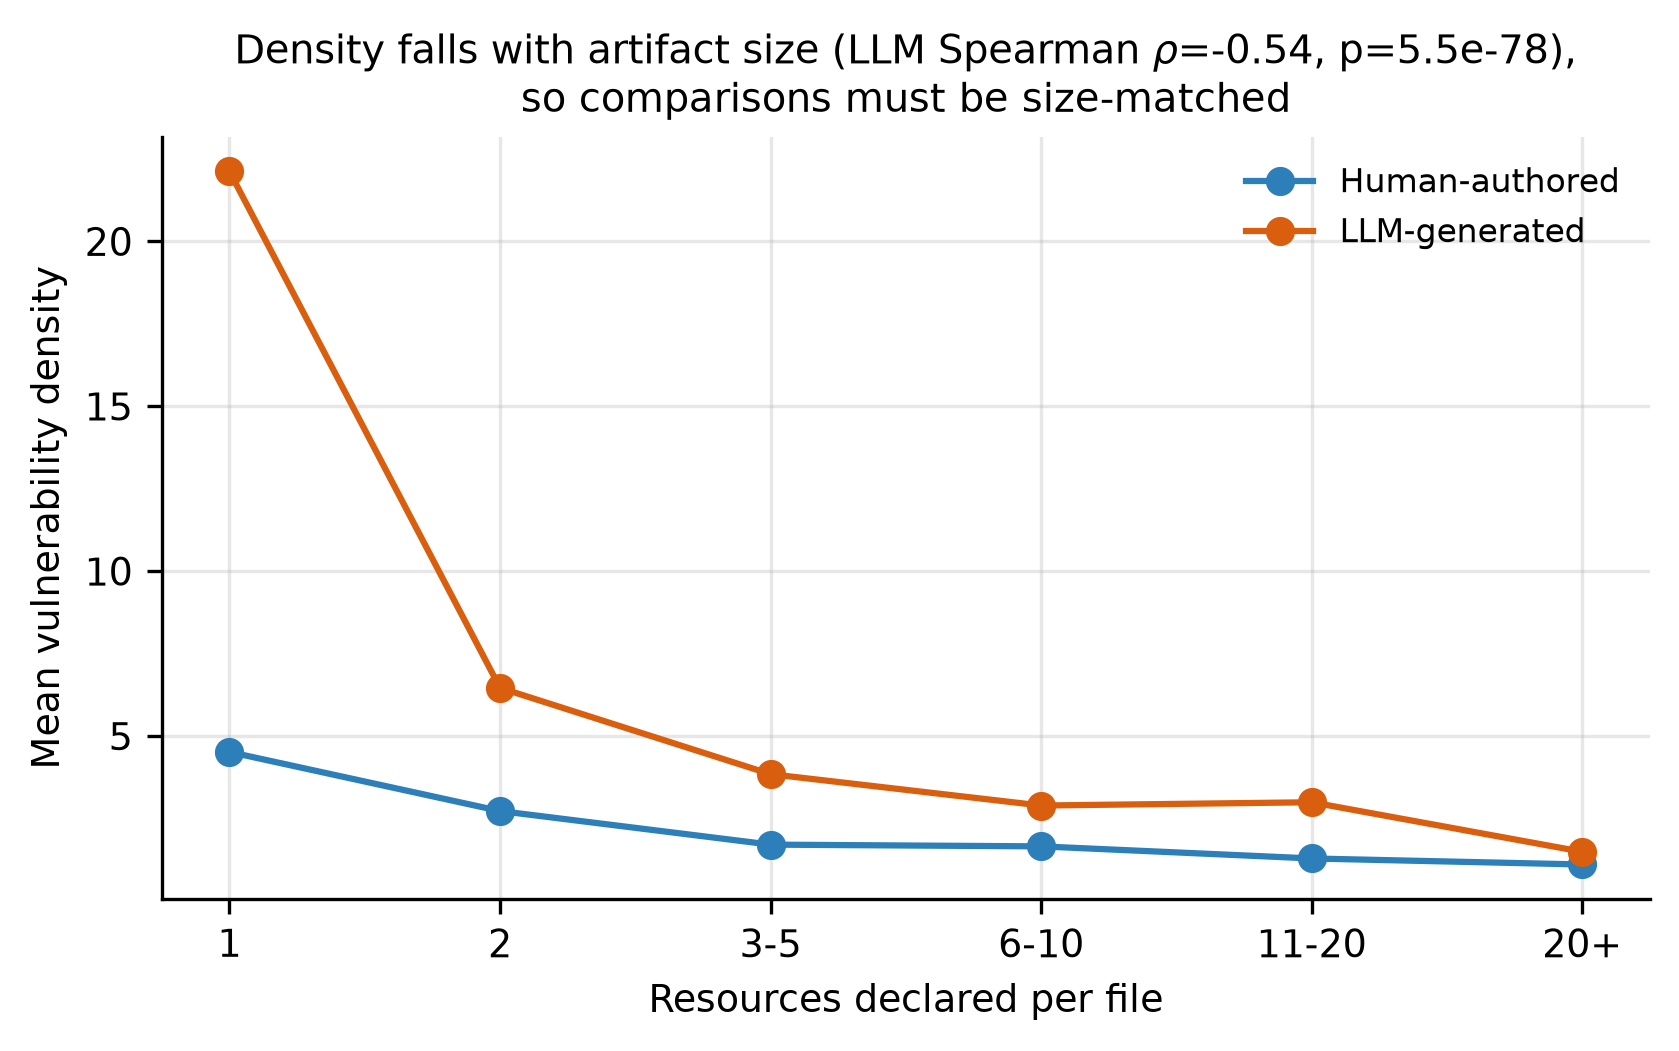
\includegraphics[width=\columnwidth]{density_vs_resources.png}
\caption{Vulnerability density declines with artifact size in both corpora,
requiring size-matched comparison.}
\label{fig:densres}
\end{figure}

\subsection{LLM-generated IaC is consistently less secure than human IaC}
\label{sec:human}
Fig.~\ref{fig:humanvsllm} compares generated and human artifacts within matched
strata. The generated corpus exhibits significantly higher density in every
stratum except the largest, with the ratio decreasing monotonically in
artifact size: $4.9\times$ at one declared resource, $2.4\times$ at two,
$2.3\times$ at three to five, $1.8\times$ at six to ten, $2.3\times$ at eleven to
twenty, and $1.4\times$ (not significant, $p=0.058$) at twenty or more.

Aggregating per configuration over shared strata (Fig.~\ref{fig:ratio}) yields a
strikingly narrow band: every configuration lies between $3.21\times$ and
$3.87\times$ the human baseline. This consistency across four vendors, open and
closed weights, and three reasoning modes suggests a property of current
LLM-generated IaC rather than of any individual model.

\begin{figure}[t]
\centering
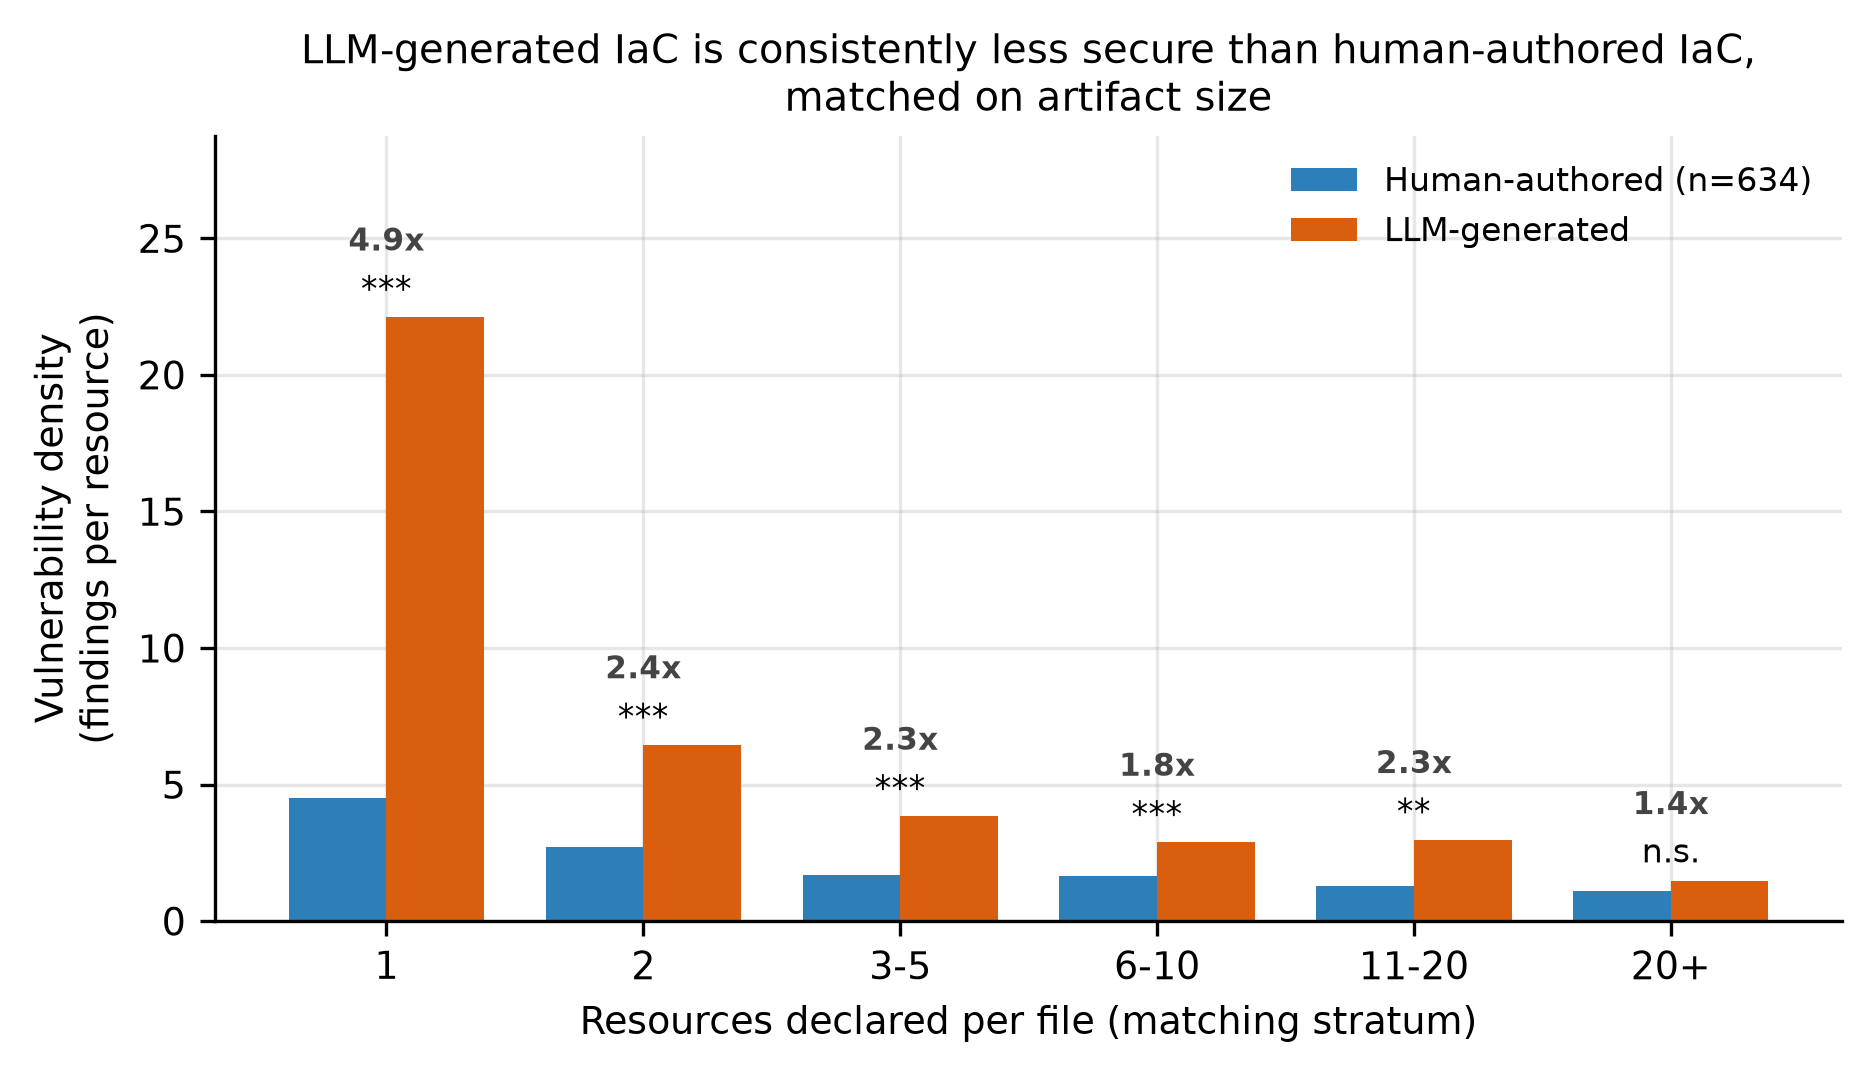
\includegraphics[width=\columnwidth]{human_vs_llm_density.png}
\caption{Size-matched comparison against the human baseline.
$^{*}p<0.05$, $^{**}p<0.01$, $^{***}p<0.001$ (Mann--Whitney $U$).}
\label{fig:humanvsllm}
\end{figure}

\begin{figure}[t]
\centering
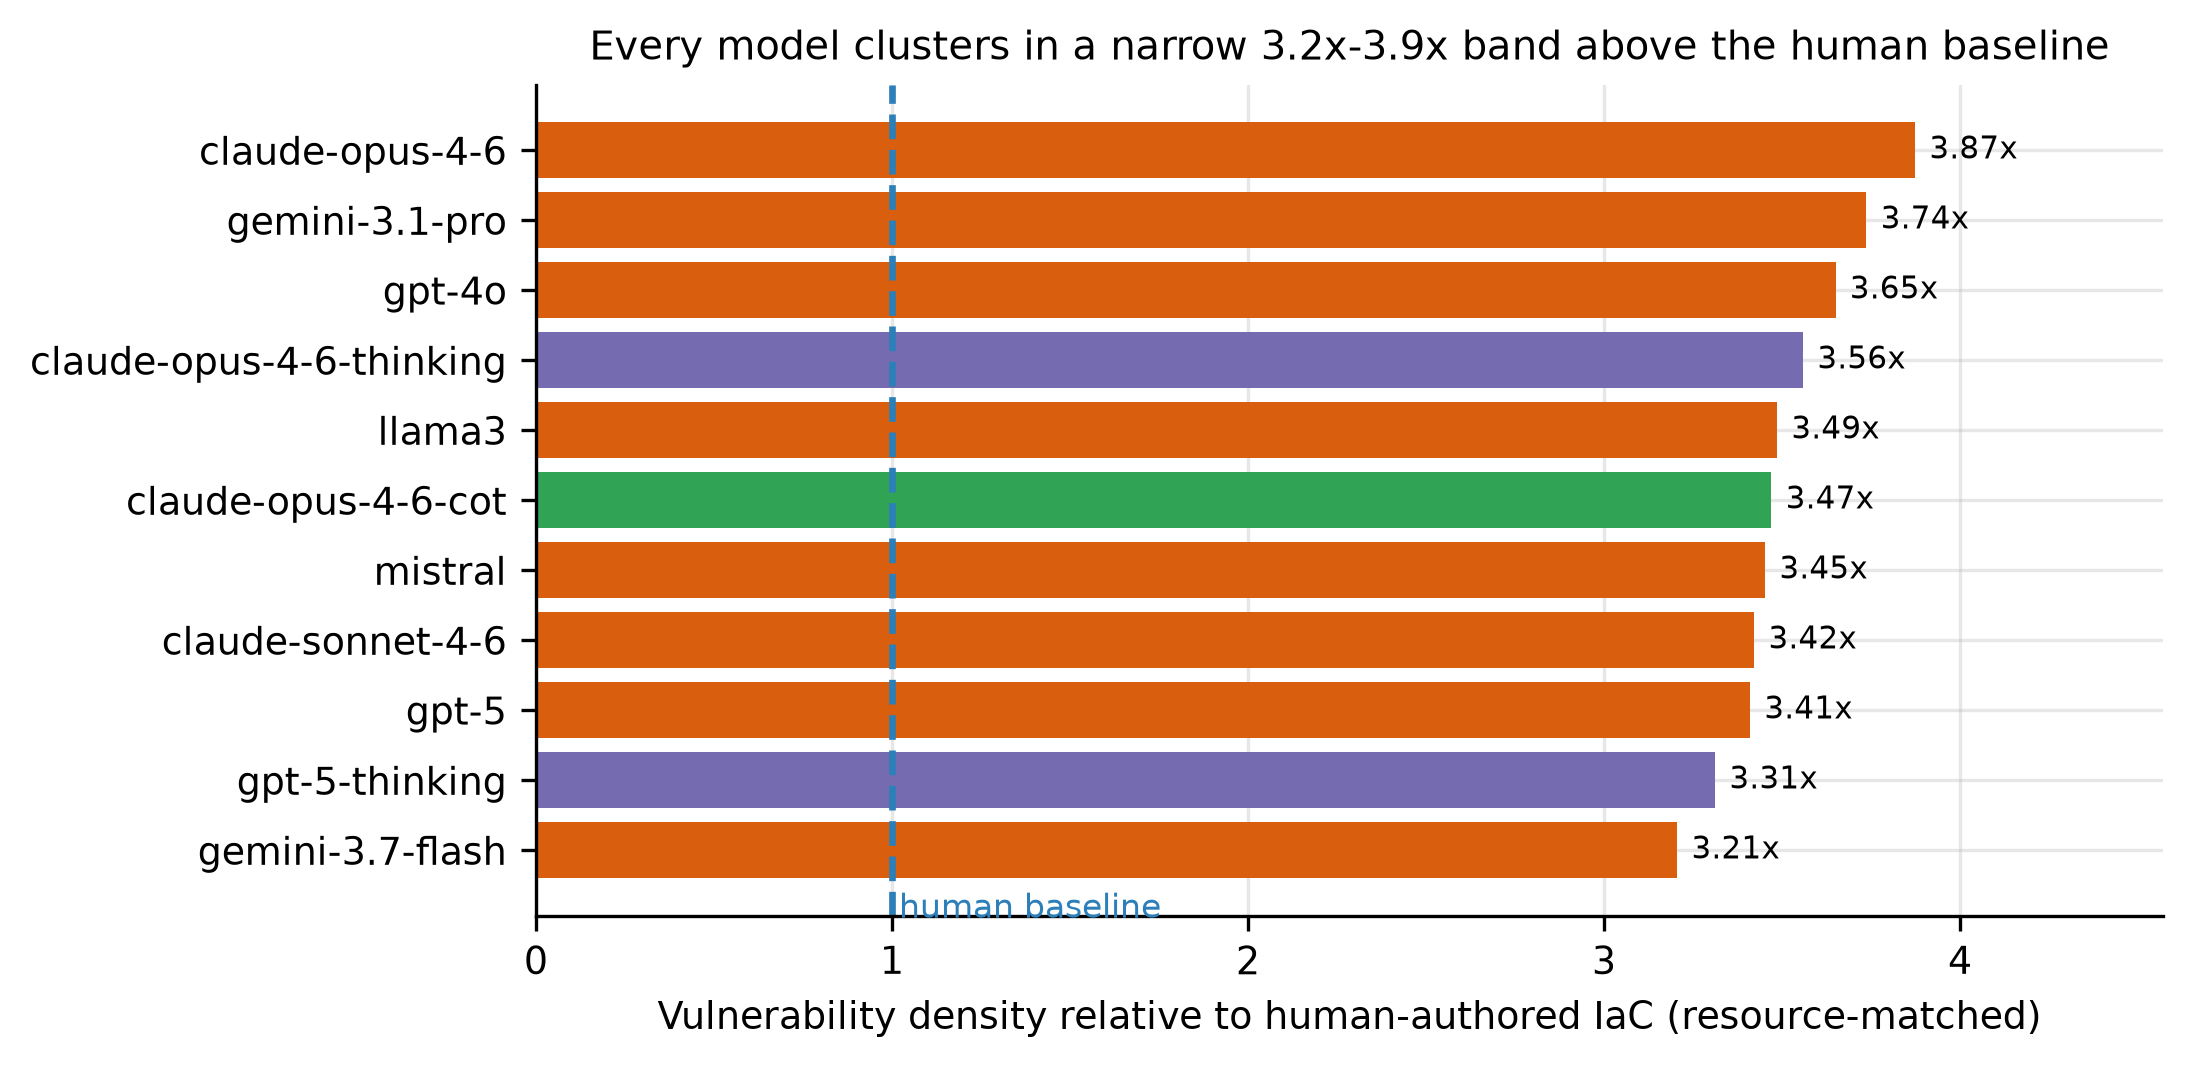
\includegraphics[width=\columnwidth]{llm_human_ratio.png}
\caption{Per-configuration density relative to the human baseline. Purple:
vendor extended thinking. Green: prompted chain-of-thought.}
\label{fig:ratio}
\end{figure}

Notably, the gap is \emph{largest on the simplest tasks}. Where a human writes a
minimal single-resource template, models emit substantially more flagged
configuration---consistent with the structural over-generation reported in
Section~\ref{sec:structural}.

\subsection{Models differ, but the classical test cannot show it}
\label{sec:omnibus}
Skillings--Mack rejects the null of equal model performance in both strata
(simple: $\chi^2=69.3$, $df=10$, $p=6.0\times10^{-11}$, 60 blocks; complex:
$\chi^2=81.2$, $df=11$, $p=8.7\times10^{-13}$, 40 blocks).

The classical alternative fails outright. Friedman requires complete blocks, and
with 12 configurations and realistic coverage gaps \emph{no scenario has every
configuration present}: complete-case analysis retains \textbf{zero} blocks in
both strata. This is not a matter of reduced power---the standard test in this
literature~\cite{demsar2006statistical} is simply uncomputable on a design of
this shape. We regard this as a transferable methodological point: multi-model
benchmarks routinely lose cells to refusals, quota limits, and truncation, and
should default to incomplete-block statistics.

\subsection{Reasoning modes}
\label{sec:reasoning}
Table~\ref{tab:reasoning} reports paired within-model contrasts on the simple
stratum, where sample size is largest. Vendor extended thinking reduces density
relative to standard generation ($-13.2\%$, $p=0.012$) and, more informatively,
relative to prompted chain-of-thought ($-12.0\%$, $p=0.0013$). Prompted
chain-of-thought alone is statistically indistinguishable from standard
generation ($-1.3\%$, $p=0.238$).

\begin{table}[t]
\caption{Paired reasoning-mode contrasts, simple stratum.}
\label{tab:reasoning}
\centering
\small
\begin{tabular}{@{}lrrr@{}}
\toprule
Contrast & $n$ & $\Delta$ density & $p$ \\
\midrule
standard $\rightarrow$ extended thinking & 60 & $-13.2\%$ & \textbf{0.012} \\
prompted CoT $\rightarrow$ extended thinking & 60 & $-12.0\%$ & \textbf{0.0013} \\
standard $\rightarrow$ prompted CoT & 60 & $-1.3\%$ & 0.238 \\
gpt-5 $\rightarrow$ \texttt{reasoning\_effort=high} & 58 & $-10.2\%$ & 0.153 \\
\bottomrule
\end{tabular}
\end{table}

Fig.~\ref{fig:contrasts} visualizes these contrasts. The practical implication is
direct: instructing a model to ``think step by step'' does not confer the
security benefit of paying for reasoning tokens. Given that prompted
chain-of-thought is often treated as a free substitute, and that its benefits
appear concentrated in mathematical and symbolic domains~\cite{sprague2025cot},
this distinction matters for practitioner guidance.

\begin{figure}[t]
\centering
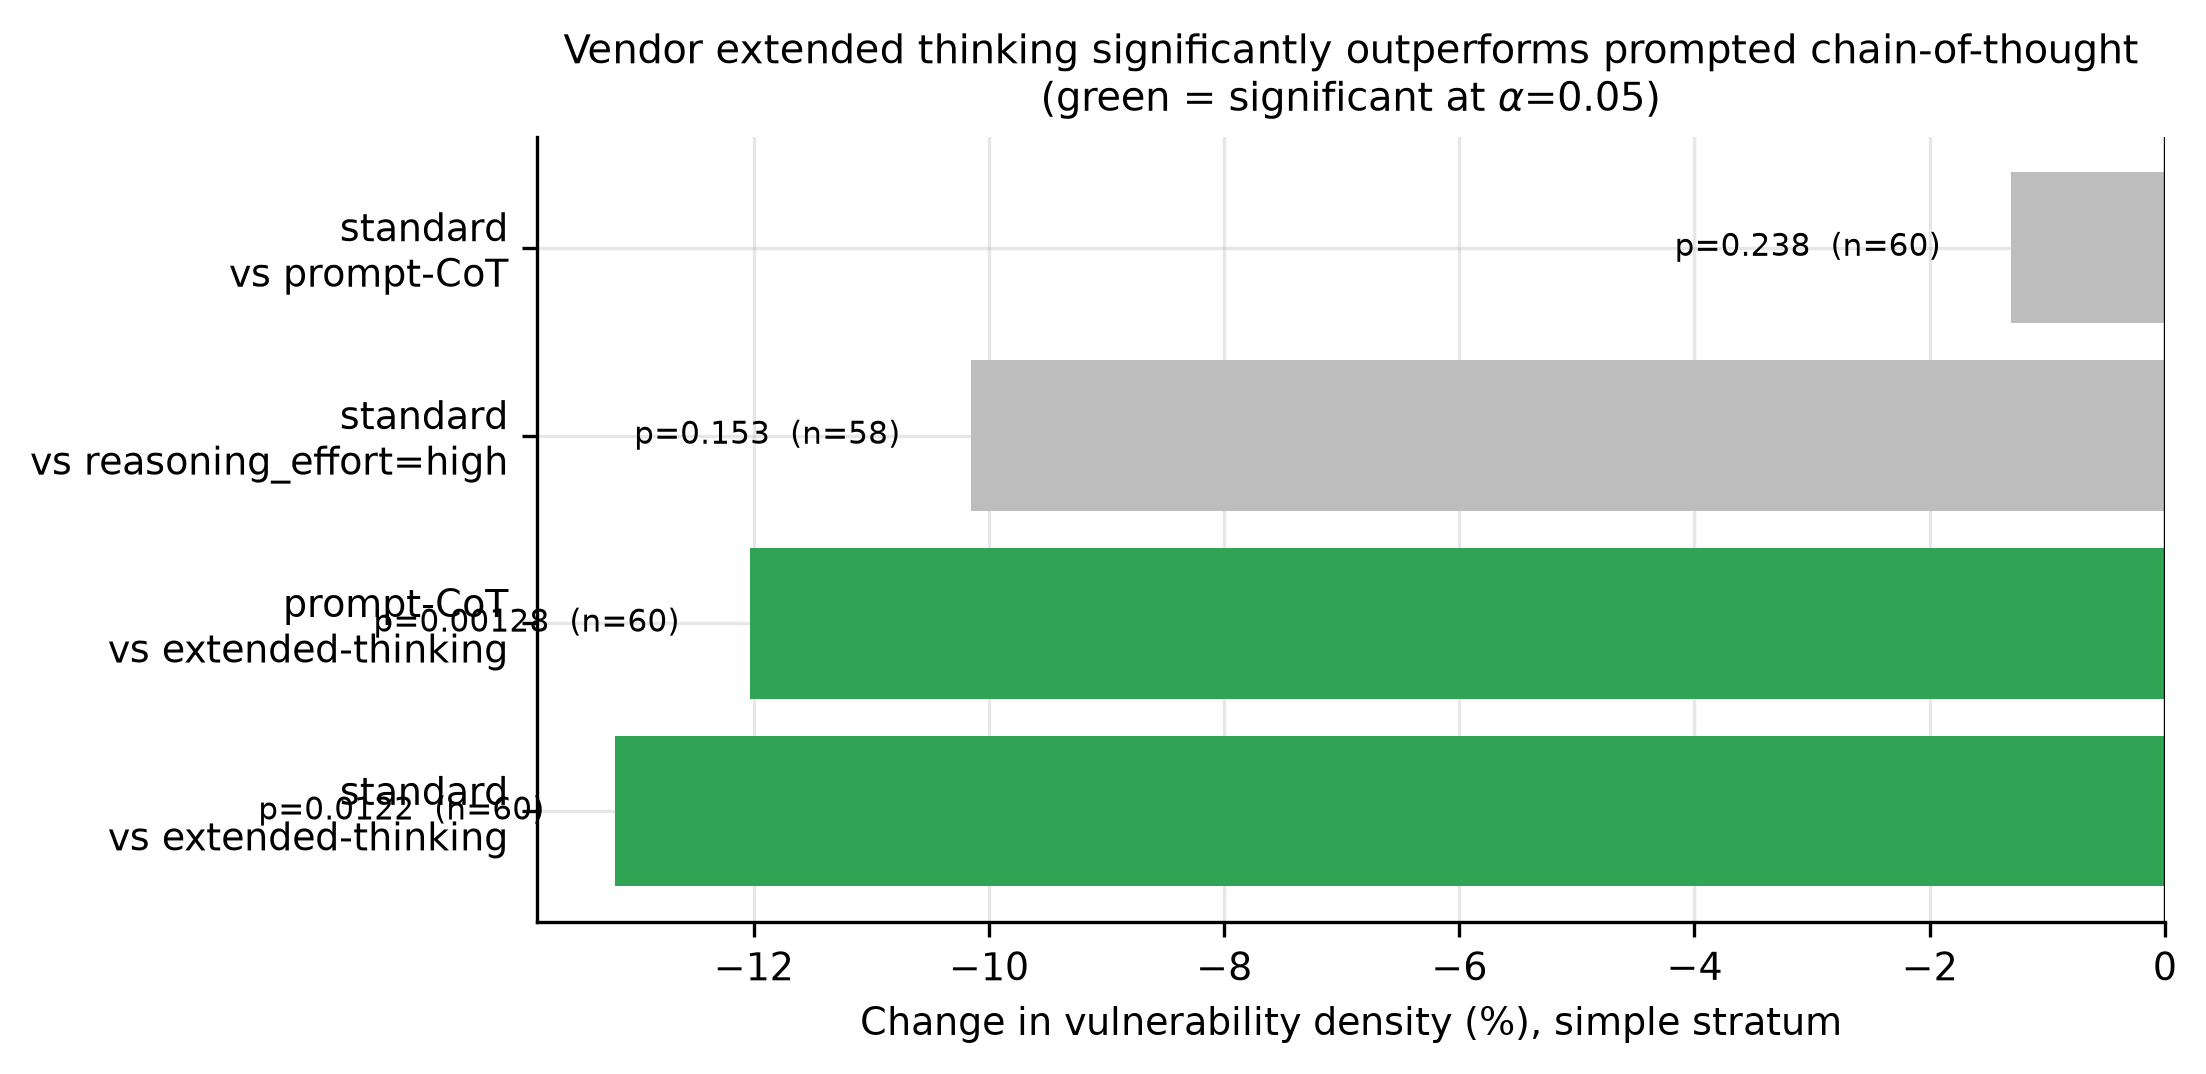
\includegraphics[width=\columnwidth]{reasoning_mode_contrasts.png}
\caption{Paired reasoning-mode contrasts on the simple stratum. Green bars are
significant at $\alpha=0.05$.}
\label{fig:contrasts}
\end{figure}

Instrumenting the API explains why the effect, though real, is bounded.
Fig.~\ref{fig:tokens} shows reasoning-token expenditure: a median of 29 tokens on
simple scenarios and 151 on complex ones, against median completion lengths of
886 and 18{,}533 tokens respectively---under $1\%$ of the output budget on
complex tasks, despite a generous configured allowance. The budget is a ceiling
the model may underspend, not a target. A modest measured effect should therefore
\emph{not} be read as ``reasoning does not help''; on this task class the
mechanism is barely exercised.

\begin{figure}[t]
\centering
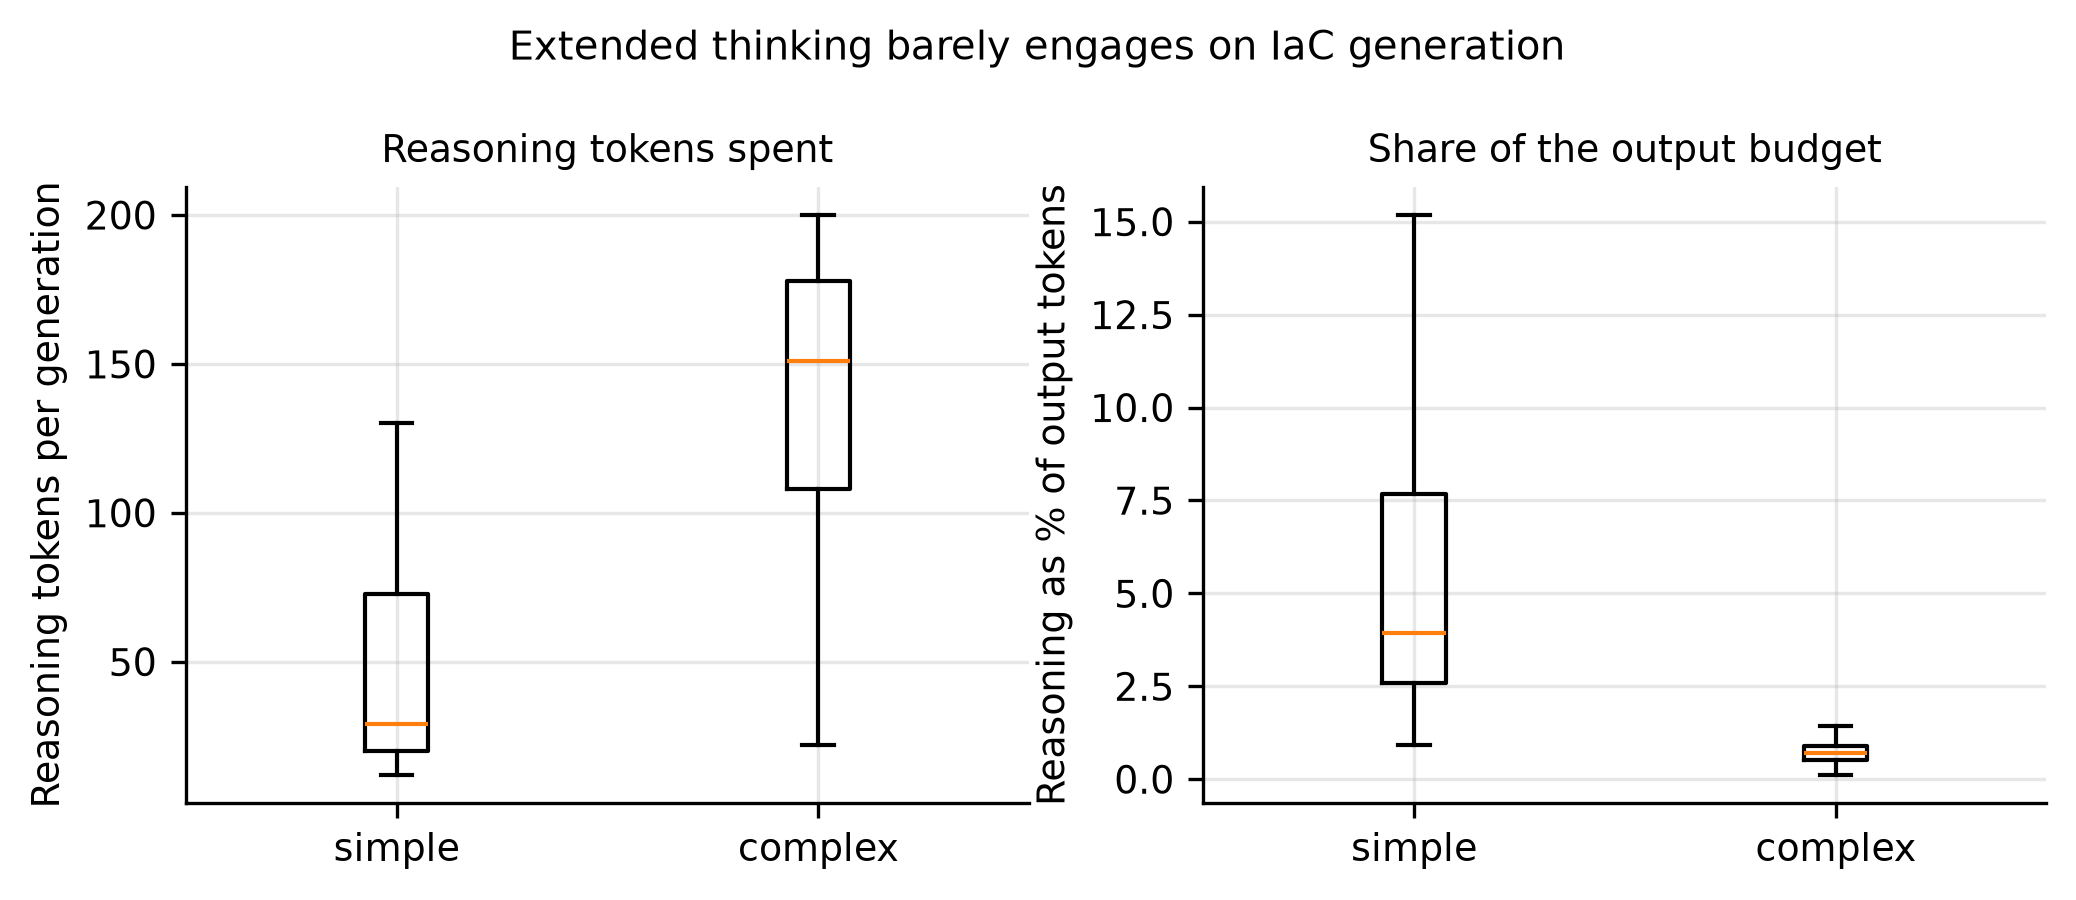
\includegraphics[width=\columnwidth]{reasoning_token_share.png}
\caption{Reasoning-token expenditure under extended thinking. The mechanism is
barely engaged on IaC generation.}
\label{fig:tokens}
\end{figure}

\subsection{Rate model}
The negative binomial GEE with exposure offset yields incidence rate ratios from
0.73 to 4.64 against a \texttt{claude-opus-4-6} reference. The prompted-CoT arm
is significantly below the reference (IRR $0.73$, 95\% CI $[0.54,0.99]$,
$p=0.041$); \texttt{phi3} is highest (IRR $4.64$, $[3.12,6.89]$,
$p=2.9\times10^{-14}$).

The \texttt{phi3} result inverts a naive reading. It records the fewest absolute
findings and appears safest by raw count, but declares almost no parseable
infrastructure; \emph{per resource} it is the worst configuration measured. This
is survivorship bias made explicit, and it is why absolute counts should not be
used for cross-model comparison.

\subsection{What models get wrong, and what the engines disagree about}
\label{sec:categories}
Mapping findings to CIS Benchmark categories~\cite{cis_benchmarks}
(Fig.~\ref{fig:cis}) shows Networking as the largest named category (4{,}554
findings), followed by Identity and Access Management (2{,}849),
Logging/Monitoring (2{,}149), and Encryption (2{,}140). A large residual
``Other'' bucket (27{,}111) is dominated by Checkov rules that do not map cleanly
onto CIS categories and is a tooling artifact rather than a vulnerability class.
The prominence of networking and IAM is consistent with the security smells
catalogued for hand-written IaC~\cite{rahman2019seven}: permissive ingress rules
and over-broad role grants remain the dominant failure modes whether the author
is human or machine.

Fig.~\ref{fig:scanner} shows per-engine finding counts. The three engines
disagree substantially in volume---Checkov and KICS report comparable totals
while Trivy reports roughly 23\% fewer---which is precisely the convergent-validity
argument for using three independent vendors. A single-engine study would
inherit that engine's rule coverage as if it were ground truth. We note that our
own earlier, partially-covered corpus would have supported different conclusions
about inter-engine agreement, which is why we report coverage explicitly.

\begin{figure}[t]
\centering

\includegraphics[width=\columnwidth]{cis_category_heatmap.png}
\caption{Findings by CIS category and configuration. ``Other'' reflects rules
without a clean CIS mapping and should not be read as a vulnerability class.}
\label{fig:cis}
\end{figure}

\begin{figure}[t]
\centering

\includegraphics[width=\columnwidth]{scanner_agreement.png}
\caption{Findings by engine. Volume disagreement across three independent
vendors motivates multi-engine evaluation.}
\label{fig:scanner}
\end{figure}

\subsection{Schema validity}
\label{sec:validity}
Schema-validity pass rates (Fig.~\ref{fig:validity}) cluster between 27\% and
35\% for all frontier configurations and collapse for the small local models
(\texttt{mistral} 8\%, \texttt{llama3} 6\%, \texttt{phi3} 5\%). The absolute
rates are low because complex scenarios demand multi-service architectures that
must satisfy real provider schemas; they are nonetheless directly comparable
across configurations, and they are what makes the survivorship correction in
Section~\ref{sec:negative} necessary.

\begin{figure}[t]
\centering
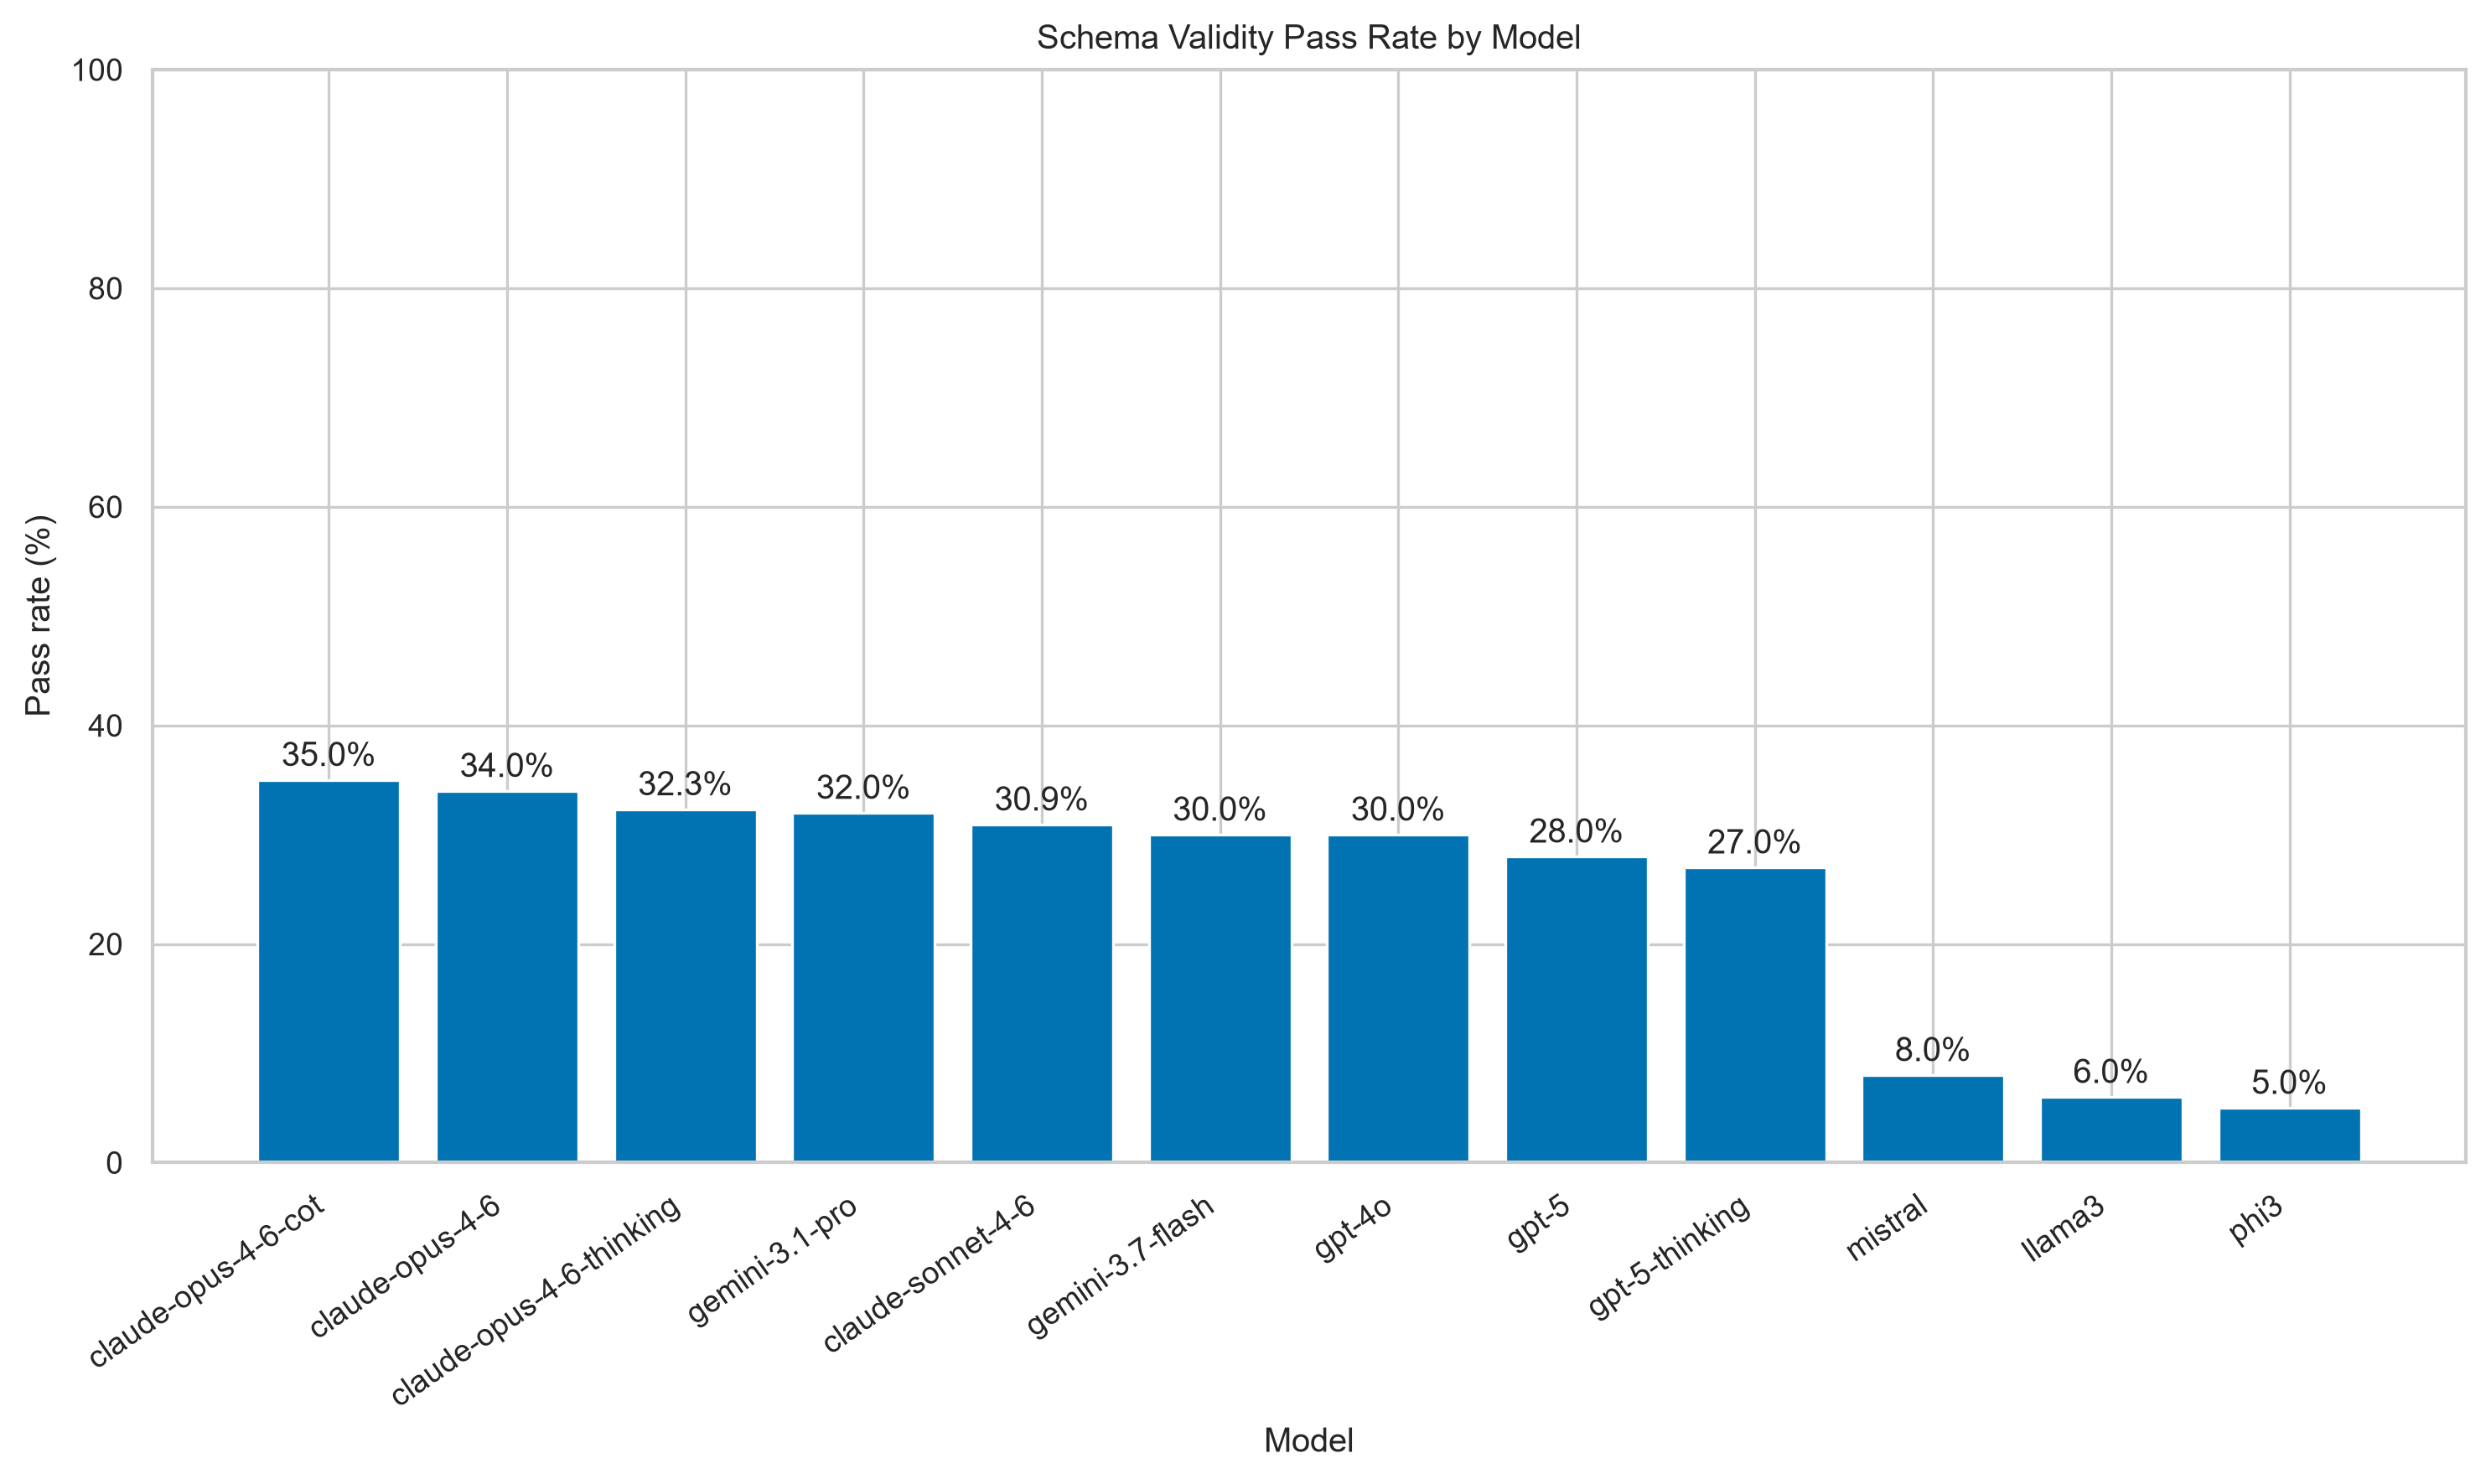
\includegraphics[width=\columnwidth]{schema_validity_pass_rate.png}
\caption{Schema-validity pass rate by configuration.}
\label{fig:validity}
\end{figure}

\subsection{Structural divergence}
\label{sec:structural}
Two-sample KS tests reject distributional equality with human-authored IaC for
every configuration on every structural metric (36/36 tests, all $p<0.05$).
Generated templates declare 13--36 resources on average against 5.31 for humans.
\texttt{gpt-4o} is closest ($D=0.160$, $p=0.021$); \texttt{phi3} is most
divergent ($D=0.990$). Models systematically over-generate infrastructure
relative to human engineers.

\subsection{Human evaluation and judge calibration}
\label{sec:human-eval}
Three cloud-security practitioners independently scored a stratified sample of
scenarios on four criteria. Inter-rater agreement (Fleiss'
$\kappa$~\cite{fleiss1971measuring}) was fair on real-world plausibility
($0.391$) and hallucination flagging ($0.266$), slight on architectural
coherence ($0.210$), and negligible on security-test relevance ($0.059$).
Under the Landis--Koch scale~\cite{landis1977measurement} the last is barely
above chance: experienced engineers do not agree on whether a scenario poses a
meaningful security decision. This is a substantive result about the difficulty
of human security evaluation, not merely a limitation of our panel.

Against the human consensus, the LLM judge is substantial on hallucination
detection (94.4\% exact, Cohen's $\kappa=0.640$~\cite{cohen1960coefficient}) and
near-perfect on plausibility (quadratic-weighted $\kappa=0.795$, 100\% within one
point), but near chance on architectural coherence ($\kappa=0.177$, 27.8\%
exact). The boundary is actionable: automated judges are usable for factual
verification, not for architectural assessment.

\subsection{Two negative results}
\label{sec:negative}
First, the intuitive \emph{validity--security} hypothesis---that models better
at producing deployable code produce more vulnerable code---is unsupported.
Across configurations, schema-validity pass rate and vulnerability density are
uncorrelated ($r=0.158$, $p=0.625$; Spearman $\rho=0.098$, $p=0.761$). Pass rates
cluster between 27\% and 35\% for all frontier configurations with no
accompanying density relationship. Only the survivorship component holds:
\texttt{phi3} passes 5\% and produces almost no parseable infrastructure.

Second, as reported in Section~\ref{sec:omnibus}, complete-case Friedman is
uncomputable on this design.

\section{Threats to Validity}
\label{sec:threats}

\textbf{Construct.} The human corpus is \emph{not} a matched control: those
templates were not written against our scenarios, and many are curated examples
rather than production infrastructure. Example templates may be deliberately
minimal, which could bias the baseline in either direction; we do not claim to
know which. Vendor reasoning mechanisms also differ (token budget versus effort
level) and are not pooled.

\textbf{Internal.} Scanner findings indicate policy deviations, not proven
exploitability; ``zero findings'' means only that three rulesets flagged nothing.
Checkov does not emit severity tiers without a commercial subscription, so
severity analysis reflects Trivy and KICS only. Scenarios were authored by a
model that also appears under test, an unquantified residual risk mitigated by
requirements-only phrasing and independent human and judge review.

\textbf{Measurement infrastructure.} During this study we identified several
defects that produced plausible-looking but incorrect results with no error
raised: a platform encoding mismatch that aborted scanning for an entire
configuration; a filename-handling rule that silently discarded one engine's
reports for configurations whose names contain a period; a schema mismatch that
caused one engine's findings to parse as zero for ten of twelve configurations;
a resource-count source that degraded to a constant denominator, inflating an
apparent effect to $+2528\%$ where the corrected value is $-14\%$; and
ungenerated scenarios being scored as zero-vulnerability. Each would have
survived review because the resulting numbers looked reasonable. We report this
explicitly: in multi-tool benchmarks, derived counts must be reconciled against
source artifacts rather than trusted, and we release coverage manifests and
regeneration scripts so that any published figure can be recomputed.

\textbf{External.} Hosted models change without notice; results describe the
configurations as accessed. Terraform dominates the corpus, and engine rule
coverage differs by format. Statistical power for the paired reasoning contrasts
is limited ($n\leq60$), and only two model families expose reasoning arms.

\section{Conclusion and Future Work}

Measured against human-authored infrastructure through an identical toolchain
and matched on artifact size, current language models produce IaC with
approximately $3.2\times$--$3.9\times$ the vulnerability density of human
engineers, with remarkable consistency across vendors and weight availability.
The gap is widest on the simplest tasks. Vendor reasoning modes deliver a real
but modest improvement and meaningfully outperform prompted chain-of-thought,
which alone provides no measurable security benefit---though the mechanism is
barely engaged on this task class, consuming under $1\%$ of output tokens.

Future work should pursue a matched human control authored against the same
scenarios; larger samples and additional model families for the reasoning
contrasts; a sensitivity sweep over reasoning-budget settings; exploitability
triage to connect policy findings to realizable attack paths; deployment-time
validation beyond static analysis; and improved rubric anchoring, given that
expert agreement on security-test relevance was near chance.

\section*{Data Availability}
The pipeline, statistical analysis code, figure generation, coverage manifests,
and threats-to-validity documentation are released. Every figure and table is
regenerated from the released data by a single command.

\bibliographystyle{IEEEtran}
\bibliography{references}

\end{document}
